%==============================================================================
% PREAMBLE
%==============================================================================
\documentclass[mathserif, xcolor=dvipsnames]{beamer}
% \usepackage{helvet}
\usepackage[T1]{fontenc}
\usepackage{amsmath, amsfonts,amsthm}
\usepackage{url}
\usepackage{courier}
\usepackage{listings}
\usepackage{color}
\definecolor{mygray}{rgb}{0.5,0.5,0.5}
\lstset{basicstyle=\footnotesize\ttfamily,language=Python,commentstyle=\color{mygray}}

\usetheme[height=10mm]{Rochester}
\usecolortheme[named=MidnightBlue]{structure}
\setbeamertemplate{navigation symbols}{}

\title{First tutorial session}
\author{Vincent Dumoulin}
\date{January 15, 2015}

%==============================================================================
% BODY
%==============================================================================
\begin{document}

%------------------------------------------------------------------------------
% TITLE
%------------------------------------------------------------------------------
\begin{frame}[plain]
    \titlepage
\end{frame}

%------------------------------------------------------------------------------
% Outline
%------------------------------------------------------------------------------
\begin{frame}
    \frametitle{Outline}
    \begin{enumerate}\addtolength{\itemsep}{1.5\baselineskip}
        \item{Solution to the numpy + MNIST + MLP assignment}
        \item{Git primer}
        \item{Theano primer}
        \item{Porting numpy + MNIST + MLP to theano + MNIST + MLP}
    \end{enumerate}
\end{frame}

%------------------------------------------------------------------------------
% Solution to numpy + MNIST + MLP
%------------------------------------------------------------------------------
\begin{frame}
    \frametitle{Solution to numpy + MNIST + MLP}

    \begin{block}{Setup}
    \begin{align*}
        \mathbf{x} &= [x_1, \cdots, x_A]^T,
        &\mathbf{t} &= [t_1, \cdots, x_C]^T, \\
        \mathbf{W} &= \begin{pmatrix}
            W_{1,1} & \cdots & W_{1,A} \\
            \cdots  & \cdots & \cdots  \\
            W_{H,1} & \cdots & W_{H,A} \\
        \end{pmatrix},
        &\mathbf{b} &= [b_1, \cdots, b_H]^T, \\
        \mathbf{V} &= \begin{pmatrix}
            V_{1,1} & \cdots & V_{1,H} \\
            \cdots  & \cdots & \cdots  \\
            V_{C,1} & \cdots & V_{C,H} \\
        \end{pmatrix},
        &\mathbf{c} &= [c_1, \cdots, c_C]^T, \\
        \mathbf{h} &= \sigma(\mathbf{W}\mathbf{x} + \mathbf{b}),
        &\mathbf{y} &= \textrm{softmax}(\mathbf{V}\mathbf{h} + \mathbf{c})
    \end{align*}

    \begin{equation*}
        \mathcal{L} = -\mathbf{t}^T \log \mathbf{y}
    \end{equation*}
    \end{block}
\end{frame}

\begin{frame}
    \frametitle{Solution to numpy + MNIST + MLP}

    \begin{block}{Derivatives}
    \begin{equation*}
    \begin{split}
        \frac{\partial \mathcal{L}}{\partial \mathbf{V}}
            &= (\mathbf{y} - \mathbf{t}) \mathbf{h}^T, \\
        \frac{\partial \mathcal{L}}{\partial \mathbf{c}}
            &= \mathbf{y} - \mathbf{t} \\
        \frac{\partial \mathcal{L}}{\partial \mathbf{W}}
            &= [\mathbf{V}^T(\mathbf{y} - \mathbf{t}) \odot \mathbf{h} \odot
                (\mathbf{1} - \mathbf{h})] \mathbf{x}^T, \\
        \frac{\partial \mathcal{L}}{\partial \mathbf{b}}
            &= \mathbf{V}^T(\mathbf{y} - \mathbf{t}) \odot \mathbf{h} \odot
               (\mathbf{1} - \mathbf{h})
    \end{split}
    \end{equation*}
    \end{block}

    \begin{alertblock}{A complete derivation can be found here}
    \url{https://raw.githubusercontent.com/vdumoulin/ift6266h15/master/assignments/01/solution.pdf}
    \end{alertblock}
\end{frame}

\begin{frame}
    \frametitle{Solution to numpy + MNIST + MLP}

    \begin{alertblock}{The full python implementation can be found here}
    \url{https://raw.githubusercontent.com/vdumoulin/ift6266h15/master/assignments/01/solution.py}
    \end{alertblock}
\end{frame}

%------------------------------------------------------------------------------
% Why version control?
%------------------------------------------------------------------------------
\begin{frame}
    \frametitle{Git primer}
    \begin{block}{Why version control?}
    \begin{itemize} \addtolength{\itemsep}{0.5\baselineskip}
        \item{A nice and clean alternative to maintaining multiple versions of
              the same file using some sort of custom naming scheme
              (\emph{e.g.} \texttt{myfile\_9.py})}
        \item{A way to end the fear of saving and quitting}
        \item{Keep a trace how your files change throughout development}
        \item{Revert back to older versions}
        \item{Manage multiple versions (\emph{branches}) of your code at the
              same time}
    \end{itemize}
    \end{block}

    \begin{alertblock}{Going further}
        \footnotesize
        \url{http://git-scm.com/book/en/v2/Getting-Started-About-Version-Control}
    \end{alertblock}
\end{frame}

%------------------------------------------------------------------------------
% What is git?
%------------------------------------------------------------------------------
\begin{frame}
    \frametitle{Git primer}
    \begin{block}{What is git?}
    \begin{itemize}\addtolength{\itemsep}{0.5\baselineskip}
        \item{Distributed version control system
              \begin{itemize}
                  \item{No checking out single files: local version fully
                        mirrors the repository}
                  \item{No central authority on what is the \emph{true}
                        codebase}
               \end{itemize}}
        \item{Takes \emph{snapshots} of the state of a repository at a given
              time}
        \item{Intelligent about not duplicating information from one snapshot
              to another}
    \end{itemize}
    \end{block}

    \begin{alertblock}{Going further}
        \footnotesize
        \url{http://git-scm.com/book/en/v2/Getting-Started-Git-Basics}
    \end{alertblock}
\end{frame}

%------------------------------------------------------------------------------
% What is Github?
%------------------------------------------------------------------------------
\begin{frame}
    \frametitle{Git primer}
    \begin{block}{What is Github?}
    \begin{itemize}\addtolength{\itemsep}{0.5\baselineskip}
        \item{A place to host your git repositories}
        \item{Makes it easy to
              \begin{itemize}
                  \item{Share code with others}
                  \item{Keep track of other people's code}
                  \item{Modify other people's code (\emph{forking})}
                  \item{Collaborate with other people on common code}
              \end{itemize}}
        \item{Technically no different from your own machine:
              \begin{itemize}
                  \item{Both can pull and push changes}
                  \item{Both host a fully functional version of your repository}
              \end{itemize}}
    \end{itemize}
    \end{block}
\end{frame}

%------------------------------------------------------------------------------
% Basic workflow using git and Github
%------------------------------------------------------------------------------
\begin{frame}
    \frametitle{Git primer}
    \begin{block}{Creating a repository on Github}
    \begin{figure}[H]
        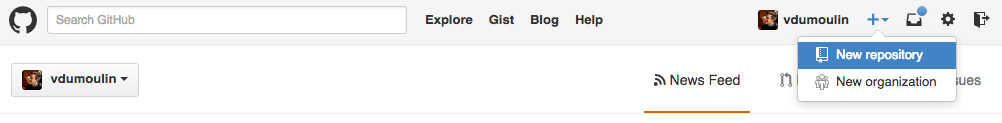
\includegraphics[width=0.75\textwidth]{repo_creation_1.png}
    \end{figure}
    \begin{figure}[H]
        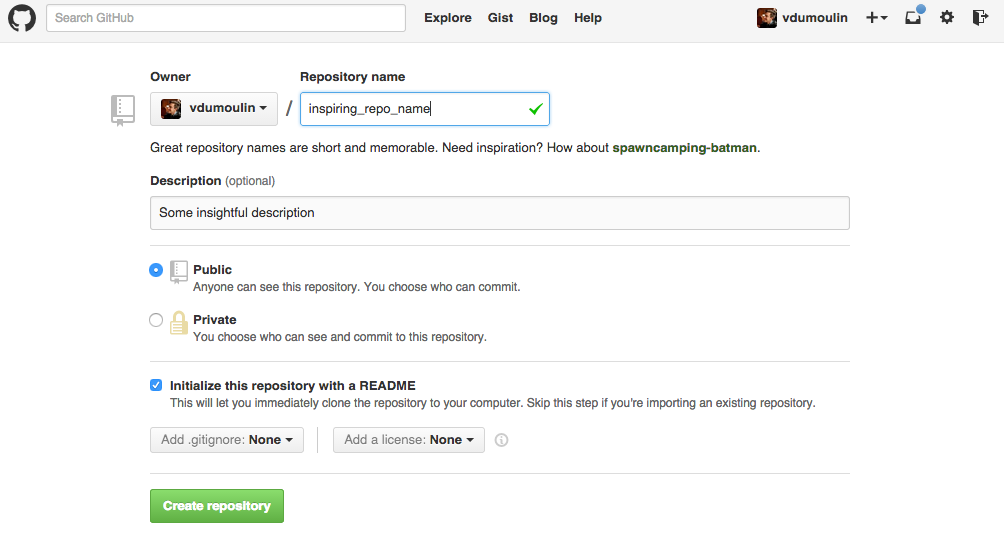
\includegraphics[width=0.75\textwidth]{repo_creation_2.png}
    \end{figure}
    \end{block}
\end{frame}

\begin{frame}[fragile]
    \frametitle{Git primer}

    \begin{block}{Identifying the repository URL}
    \begin{figure}[H]
        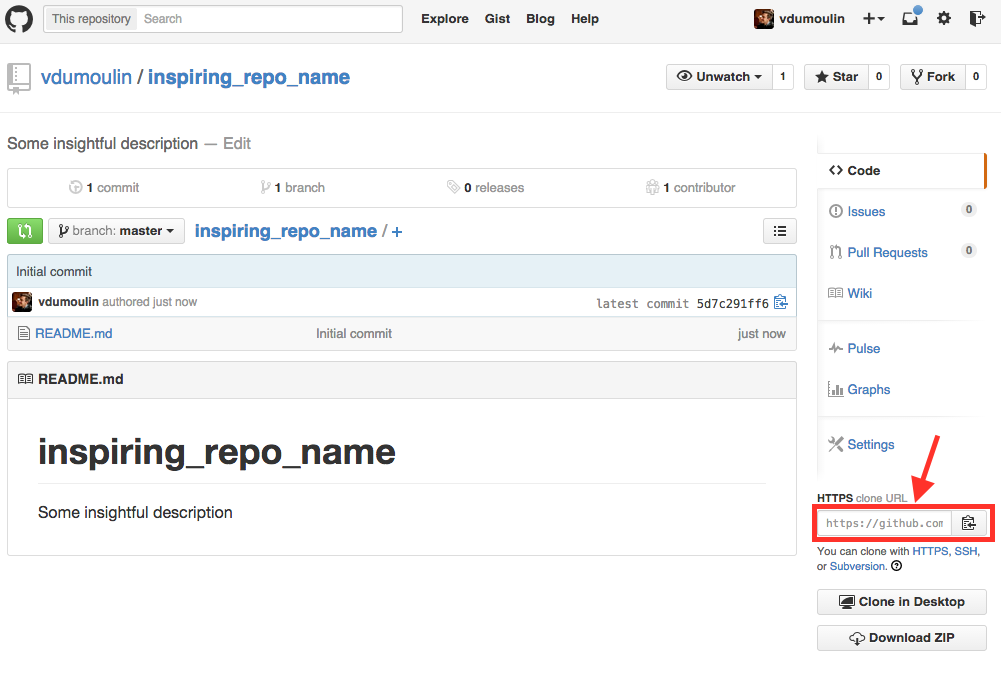
\includegraphics[width=0.5\textwidth]{repo_cloning.png}
    \end{figure}
    \end{block}

    \begin{block}{Cloning a git repository}
\begin{lstlisting}
> git clone <REPO URL>
\end{lstlisting}
    \end{block}
\end{frame}

\begin{frame}[fragile]
    \frametitle{Git primer}
    \begin{block}{Putting a file under version control}
    \begin{itemize}
        \item{Create a dummy file}
        \item{Check the status of the repository:
\begin{lstlisting}
> git status
\end{lstlisting}}
        \item{Add the file to version control:
\begin{lstlisting}
> git add my_dummy_file.py
\end{lstlisting}}
        \item{Commit the newly-added file:
\begin{lstlisting}
> git commit -m "Add new dummy file to repository"
\end{lstlisting}}
    \end{itemize}
    \end{block}
\end{frame}

\begin{frame}[fragile]
    \frametitle{Git primer}
    \begin{block}{Commit changes to a file}
    \begin{itemize}
        \item{Change something in your file}
        \item{Stage the changes:
\begin{lstlisting}
> git add my_dummy_file.py
\end{lstlisting}}
        \item{Commit the changes:
\begin{lstlisting}
> git commit -m "Add stuff to dummy file"
\end{lstlisting}}
    \end{itemize}
    \end{block}
\end{frame}

\begin{frame}[fragile]
    \frametitle{Git primer}
    \begin{block}{Pull changes on Github}
    \begin{itemize}
        \item{Run
\begin{lstlisting}
> git pull origin master
\end{lstlisting}}
    \end{itemize}
    \end{block}

    \begin{block}{Push changes on Github}
    \begin{itemize}
        \item{Pull the latest changes from your Github repo:
\begin{lstlisting}
> git pull origin master
\end{lstlisting}}
        \item{Push your changes to Github:
\begin{lstlisting}
> git push origin master
\end{lstlisting}}
    \end{itemize}
    \end{block}
\end{frame}

%------------------------------------------------------------------------------
% For more information
%------------------------------------------------------------------------------
\begin{frame}
    \frametitle{Git primer}
    \begin{alertblock}{Going further with Git}
    \url{http://git-scm.com/book/en/v2}
    \end{alertblock}
\end{frame}

%------------------------------------------------------------------------------
% What is Theano?
%------------------------------------------------------------------------------
\begin{frame}
    \frametitle{Theano primer}
    \begin{block}{What is Theano?}
    \begin{itemize}
    \item{From Theano's online documentation:
        \begin{quote}
            Theano is a Python library that allows you to define, optimize,
            and evaluate mathematical expressions involving multi-dimensional
            arrays efficiently.
        \end{quote}}
    \item{Does \emph{symbolic} computation \textbf{and} differentiation
          (\emph{i.e.} the end result of differentiation is itself a symbolic
          expression)}
    \item{Very similar to numpy with respect to its interface}
    \item{Allows doing numerical computation in a high-level language (Python)
          while still retaining the speed of low-level languages (like C)}
    \item{Allows the generation of efficient CPU and GPU code transparently}
    \end{itemize}
    \end{block}
\end{frame}

%------------------------------------------------------------------------------
% Typical Theano workflow
%------------------------------------------------------------------------------
\begin{frame}
    \frametitle{Theano primer}
    \begin{block}{Typical Theano workflow}
    \begin{enumerate}\addtolength{\itemsep}{1.0\baselineskip}
        \item{Instantiate symbolic variables}
        \item{Build a computation graph out of those variables}
        \item{Compile a function with the symbolic variables as input and the
              output of the computation graph as output}
        \item{Call the compiled function with numerical inputs}
    \end{enumerate}
    \end{block}
\end{frame}

%------------------------------------------------------------------------------
% Theano vs. numpy
%------------------------------------------------------------------------------
\begin{frame}
    \frametitle{Theano primer}
    \begin{block}{Theano vs. numpy}
    \begin{itemize}\addtolength{\itemsep}{1.0\baselineskip}
        \item{Theano interface is \emph{very} similar to numpy interface}
        \item{numpy arrays are automatically converted to constant symbolic
              variables when used inside a computation graph}
        \item{You can manipulate Theano symbolic variables in the same way you'd
              manipulate numpy arrays}
    \end{itemize}
    \end{block}


    \begin{alertblock}{Going further: Theano's basic interface}
        \url{http://deeplearning.net/software/theano/library/tensor/basic.html}
    \end{alertblock}
\end{frame}

%------------------------------------------------------------------------------
% Types of symbolic variables
%------------------------------------------------------------------------------
\begin{frame}
    \frametitle{Theano primer}
    \begin{block}{Types of symbolic variables}
    \begin{description}\addtolength{\itemsep}{1.0\baselineskip}
        \item[TensorVariable]{Its value is unspecified at graph creation and
                              can change from one call of the compiled function
                              to another (\emph{e.g.} $x$ and $y$ in
                              $y = 3x - 2$)}
        \item[TensorConstant]{Its value is specified at graph creation and
                              does \textbf{not} change from one call of the
                              compiled funtion to another (\emph{e.g.} $3$ and
                              $-2$ in $y = 3x - 2$)}
        \item[TensorSharedVariable]{Its value is specified at graph creation
                                    but is bound to change from one call of the
                                    compiled function to another (\emph{e.g.}
                                    $a$ and $b$ in $y = ax + b$ in a regression
                                    setting where some $x$ and $y$ pairs have
                                    been observed)}
    \end{description}
    \end{block}
\end{frame}

%------------------------------------------------------------------------------
% Starting example: simple algebra
%------------------------------------------------------------------------------
\begin{frame}[fragile]
    \frametitle{Theano primer}
    \begin{examples}
\begin{lstlisting}[caption=Simple algebra]
import theano
import theano.tensor as T

# 1. Instantiate symbolic variables
x = T.vector(name='x')
y = T.vector(name='y')

# 2. Build a computation graph
z = x + y

# 3. Compile a callable function
f = theano.function(inputs=[x, y], outputs=z)

# 4. Call the function using numerical inputs
print f([1, 2], [3, 4])
\end{lstlisting}
    \end{examples}
\end{frame}

%------------------------------------------------------------------------------
% Differentiation
%------------------------------------------------------------------------------
\begin{frame}[fragile]
    \frametitle{Theano primer}
    \begin{examples}
\begin{lstlisting}[caption=Gradient computation]
import theano
import theano.tensor as T

# 1. Instantiate symbolic variables
x = T.vector(name='x')

# 2. Build a computation graph
z = (x ** 2).sum()
d_z_d_x = T.grad(z, x)

# 3. Compile a callable function
f = theano.function(inputs=[x], outputs=d_z_d_x)

# 4. Call the function using numerical inputs
print f([1, 2])
\end{lstlisting}
    \end{examples}
\end{frame}

%------------------------------------------------------------------------------
% Summary
%------------------------------------------------------------------------------
\begin{frame}[fragile]
    \frametitle{Theano primer}
    \begin{examples}
\begin{lstlisting}[caption=Linear regression]
import theano
import theano.tensor as T

x = T.scalar(name='x'); t = T.scalar(name='t')
a = theano.shared(-1.0, name='a')
b = theano.shared(0.0, name='b')

y = a * x + b
mse = (y - t) ** 2
grad_a, grad_b = T.grad(mse, [a, b])

f = theano.function(inputs=[x, t], outputs=mse,
                    updates={a: a - 0.01 * grad_a,
                             b: b - 0.01 * grad_b})

print [f(1, 5)) for i in xrange(10)]
\end{lstlisting}
    \end{examples}
\end{frame}

%------------------------------------------------------------------------------
% For more information
%------------------------------------------------------------------------------
\begin{frame}
    \frametitle{Going further}
    \begin{alertblock}{Going further: online Theano tutorial}
    \url{http://deeplearning.net/software/theano/tutorial/index.html\#tutorial}
    \end{alertblock}
\end{frame}

\end{document}
